\chapter{Aplikacja}

\section{Motywacja}

Analiza podatności pokazała, że większość wektorów ataku na ekosystem Dockera pochodzi z~błędów konfiguracji demona i~kontenerów Dockera, a~także z~błędów ludzkich związanych z~wielousługową metodą wdrażania oprogramowania. Wsparcie ze strony twórców Dockera pozwala na szybkie łatanie podatności środowiska. Jednakże aplikowanie aktualizacji bezpieczeństwa nadal jest zależne od użytkownika końcowego.

Błędy konfiguracyjne mogą pojawić się na wielu etapach pracy z~ekosystemem Dockera. Pomijając zewnętrzne zależności można wyróżnić takie elementy środowiska jak pliki konfiguracyjne demona Dockera, uprawnienia powiązanych z~nim plików i~katalogów systemu gospodarza oraz opcje przekazane przez użytkownika w~trakcie uruchomienia demona. Ponadto, konfiguracja kontenerów jest podatna na błędy wynikające z~wykorzystania nieodpowiednich dyrektyw w~plikach Dockerfile lub opcji użytych w~trakcie uruchamiania kontenerów. Polityka bezpieczeństwa powinna brać pod uwagę scenariusz w~jakim jest aplikowana i~być odpowiednio dostosowywana w~celu osiągnięcia zamierzonych celów.

Popularność Dockera dała wielu programistom dostęp do bardzo złożonego narzędzia jakim są kontenery. Jednakże, nie każdy użytkownik Dockera jest specjalistą od spraw bezpieczeństwa systemów komputerowych. Wiąże się to z~tworzeniem podatności wynikających z~nieznajomości pewnych aspektów wykorzystywanej technologii. Celem twórców wszystkich elementów ekosystemu Dockera powinno być wsparcie użytkowników w~kwestiach zwiększania bezpieczeństwa tworzonych przez nich aplikacji kontenerowych. 

Wspomniany w~poprzednich rozdziałach Docker Benchmark \cite{CISDockerBenchmark} został przeanalizowany przez twórców Dockera w~celu stworzenia narzędzia weryfikującego wykorzystanie zalecanych dobrych praktyk. Wynikiem tej pracy jest implementacja skryptu Docker Bench for Security. W~sposób statyczny analizuje on konfigurację demona i~kontenerów Dockera sprawdzając spełnienie zaleceń oznaczonych w~Docker Benchmark jako "Scored" (88/115 wszystkich zaleceń) \cite{DockerBenchSecurity}.

W ramach pracy zaprojektowano aplikację wspomagającą zautomatyzowaną analizę kontenerów Dockera pod kątem wykrywania przydziału zbyt dużej ilości uprawnień. W~porównaniu do skryptu Docker Bench for Security \cite{DockerBenchSecurity} aplikacja analizuje wykorzystanie uprawnień w~trakcie działania kontenera. Wynikiem uruchomienia aplikacji jest raport przedstawiający porównanie zadeklarowanych w~konfiguracji uprawnień kontenera z~rzeczywiście użytymi uprawnieniami. Tym samym, daje to użytkownikowi możliwość zmniejszenia wektora ataku, którym są nadmiarowe uprawnienia. W~kolejnych podrozdziałach aplikacja jest zwana również analizatorem.

\section{Wykorzystane narzędzia}

\subsection{Berkeley Packet Filter}

Filtry BPF wywodzą się z~systemu BSD (Berkeley Software Distribution), jednak obecnie dostępne są w~większości dystrybucji opartych o~system operacyjny Unix. Filtry zapewniają interfejs warstwy łącza danych w~postaci pseudo-urządzeń. Procesy przestrzeni użytkownika mogą uruchamiać program filtrujący, określający jakie pakiety mają zostać przez niego otrzymane. 

Filtry implementuje się w~postaci kodu bajtowego dla maszyny wirtualnej BPF (maszyna wirtualna BPF nie ma nic wspólnego z~opisywanymi wcześniej maszynami wirtualnymi, służącymi do wirtualizacji systemów operacyjnych). Kompilator nakłada pewne ograniczenia dotyczące kodu bajtowego BPF: skoki są możliwe tylko w~przód, zabronione jest używanie pętli, a~wyjściowy kod bajtowy może zawierać maksymalnie 4096 linii kodu. Wszystko to ma na celu zapewnienie zakończenia programu filtra, który jest uruchamiany dla każdego pakietu przychodzącego i~wychodzącego z~danego gniazda \cite{BSDPacketFilter}.

\subsection{Extended Berkeley Packet Filter}

Extended Berkeley Packet Filter rozszerzają zastosowanie maszyny wirtualnej BPF poprzez umożliwienie uruchomienia filtra na zdarzeniach innych niż przepływ pakietów. Przy pomocy eBPF możliwe jest również śledzenie (ang.~tracing) operacji wejścia/wyjścia, systemu plików, opóźnień systemu, użycia procesora, zmian stosu oraz co ważne, wywołań systemowych. Wszystkie zdarzenia są podzielone na 4 główne kategorie:
\begin{itemize}
    \item kprobes -- dynamiczne śledzenie jądra
    \item uprobes -- dynamiczne śledzenie przestrzeni użytkownika
    \item tracepoints -- statyczne śledzenie jądra
    \item perf\_events -- próbkowanie okresowe i~Performance Monitoring Counters
\end{itemize}
Tym samym filtry eBPF świetnie nadają się do tworzenia narzędzi, które w~przyszłości mają zastąpić obecnie istniejące moduły jądra. Ma to na celu postępującą transformację jądra Linuxa do architektury mikrojądra, w~której większość funkcjonalności zdefiniowana i~uruchamiana jest w~przestrzeni użytkownika. Takie podejście eliminuje część z~wad modułów, t.j. potrzebę rekompilacji jądra po ich instalacji oraz możliwość zatrzymania jądra po błędzie modułu \cite{GreggEBPF}.

Programy eBPF wymagają jądra Linuxa w~wersji przynajmniej 4.1, a~wraz z~kolejnymi wersjami jądra pojawiają się dodatkowe funkcjonalności. Przykładowo, wersja 4.7 jądra pozwala na statyczne śledzenie jądra przy pomocy rozwiązania \textit{tracepoints}. Co więcej, pisanie programów eBPF nie różni się wiele od pisania filtrów BPF -- składnia kodu bajtowego jest bardzo niskopoziomowa oraz posiada wspomniane wcześniej ograniczenia. Powoduje to wolną adopcję tego rozwiązania w~przenoszeniu modułów jądra na programy przestrzeni użytkownika \cite{JacksonEBPF}.

\subsection{BPF Compiler Collection}

Berkeley Packet Filter Compiler Collection, w~skrócie BCC, w~znacznym stopniu ułatwia pisanie programów eBPF poprzez opakowanie kodu bajtowego BPF wewnątrz programów napisanych w~języku C++ oraz udostępnienie interfejsów programistycznych w~językach Lua i~Python. Dodatkowo, repozytorium BCC zawiera dużą ilość przykładów i~wbudowanych narzędzi (ponad 150) ułatwiających nowym programistom rozpoczęcie tworzenia własnych programów.

BCC dodatkowo analizuje kod programów napisanych w~C++ dzięki czemu gwarantuje, że końcowy kod bajtowy BPF będzie poprawny. To narzędzie ma na celu zapewnienie interfejsu, który pozwoli na tworzenie tylko i~wyłącznie poprawnych programów eBPF, zachowując równocześnie dostęp do wszystkich funkcjonalności. Ponadto, minimalizuje czas spędzony na przygotowaniu i~kompilacji kodu bajtowego BPF. Umożliwia tym samym skupienie się na tworzeniu docelowej aplikacji \cite{BCCReadme}.

\subsection{Python 3.7}

Python jest interpretowanym językiem programowania wysokiego poziomu z~dynamiczną semantyką. Wbudowane wysokopoziomowe struktury w~połączeniu z~dynamicznym typowaniem i~wiązaniem czynią go idealnym kandydatem do szybkiego rozwoju oprogramowania, a~także tworzenia skryptów oraz łączenia istnięjących komponentów większego systemu \cite{PythonExecutiveSummary}.

Wersja 3.7 Pythona dostarcza wiele funkcjonalności przydatnych w~tworzeniu analizatora. Ulepszone annotacje typów i~wbudowany w~bibliotekę standardową moduł \textit{dataclasses} ułatwia tworzenie czystego kodu. Dodanie słów kluczowych \textit{async} i~\textit{await} sprawia, że Python natywnie wspiera asynchroniczność. Stworzona aplikacja w~dużym stopniu wykorzystuje również moduł \textit{threading} udostępniający klasę \textit{Thread} dla programów wielowątkowych oraz moduł \textit{queue} implementujący synchronizowaną kolejkę \cite{Python3.7}.

\subsection{Docker SDK for Python}

Docker SDK for Python jest biblioteką języka Python opakowującą interfejs programistyczny silnika Dockera. Umożliwia ona osiągnięcie wszystkiego na co pozwala również komenda \textit{docker}, jednak z~poziomu aplikacji Pythonowej, t.j. tworzenie obrazów, uruchomienie i~zarządzanie kontenerami, wsparcie dla Docker Swarm, itp. W~celu komunikacji z~demonem Dockera należy stworzyć obiekt klasy \textit{DockerClient}, który wspiera operacje synchroniczne oraz asynchroniczne \cite{PythonDockerSDK}.

\section{Schemat działania}

Działanie analizatora można przedstawić na podstawie uproszczonego algorytmu składającego się z~5 kroków:
\begin{enumerate}
    \item parsowanie argumentów linii poleceń
    \item rozpoczęcie śledzenia wywołań systemowych
    \item uruchomienie kontenera
    \item rozpoczęcie analizy wywołań systemowych
    \item zwolnienie zasobów i~zakończenie programu
\end{enumerate}
Uproszczony schemat przepływu sterowania i~przepływu danych w~analizatorze został przedstawiony na rysunku \ref{fig:analyzerFlow}. Kolejne podrozdziały opisują bardziej szczegółowo poszczególne kroki.

\begin{figure}[ht]
    \centering
    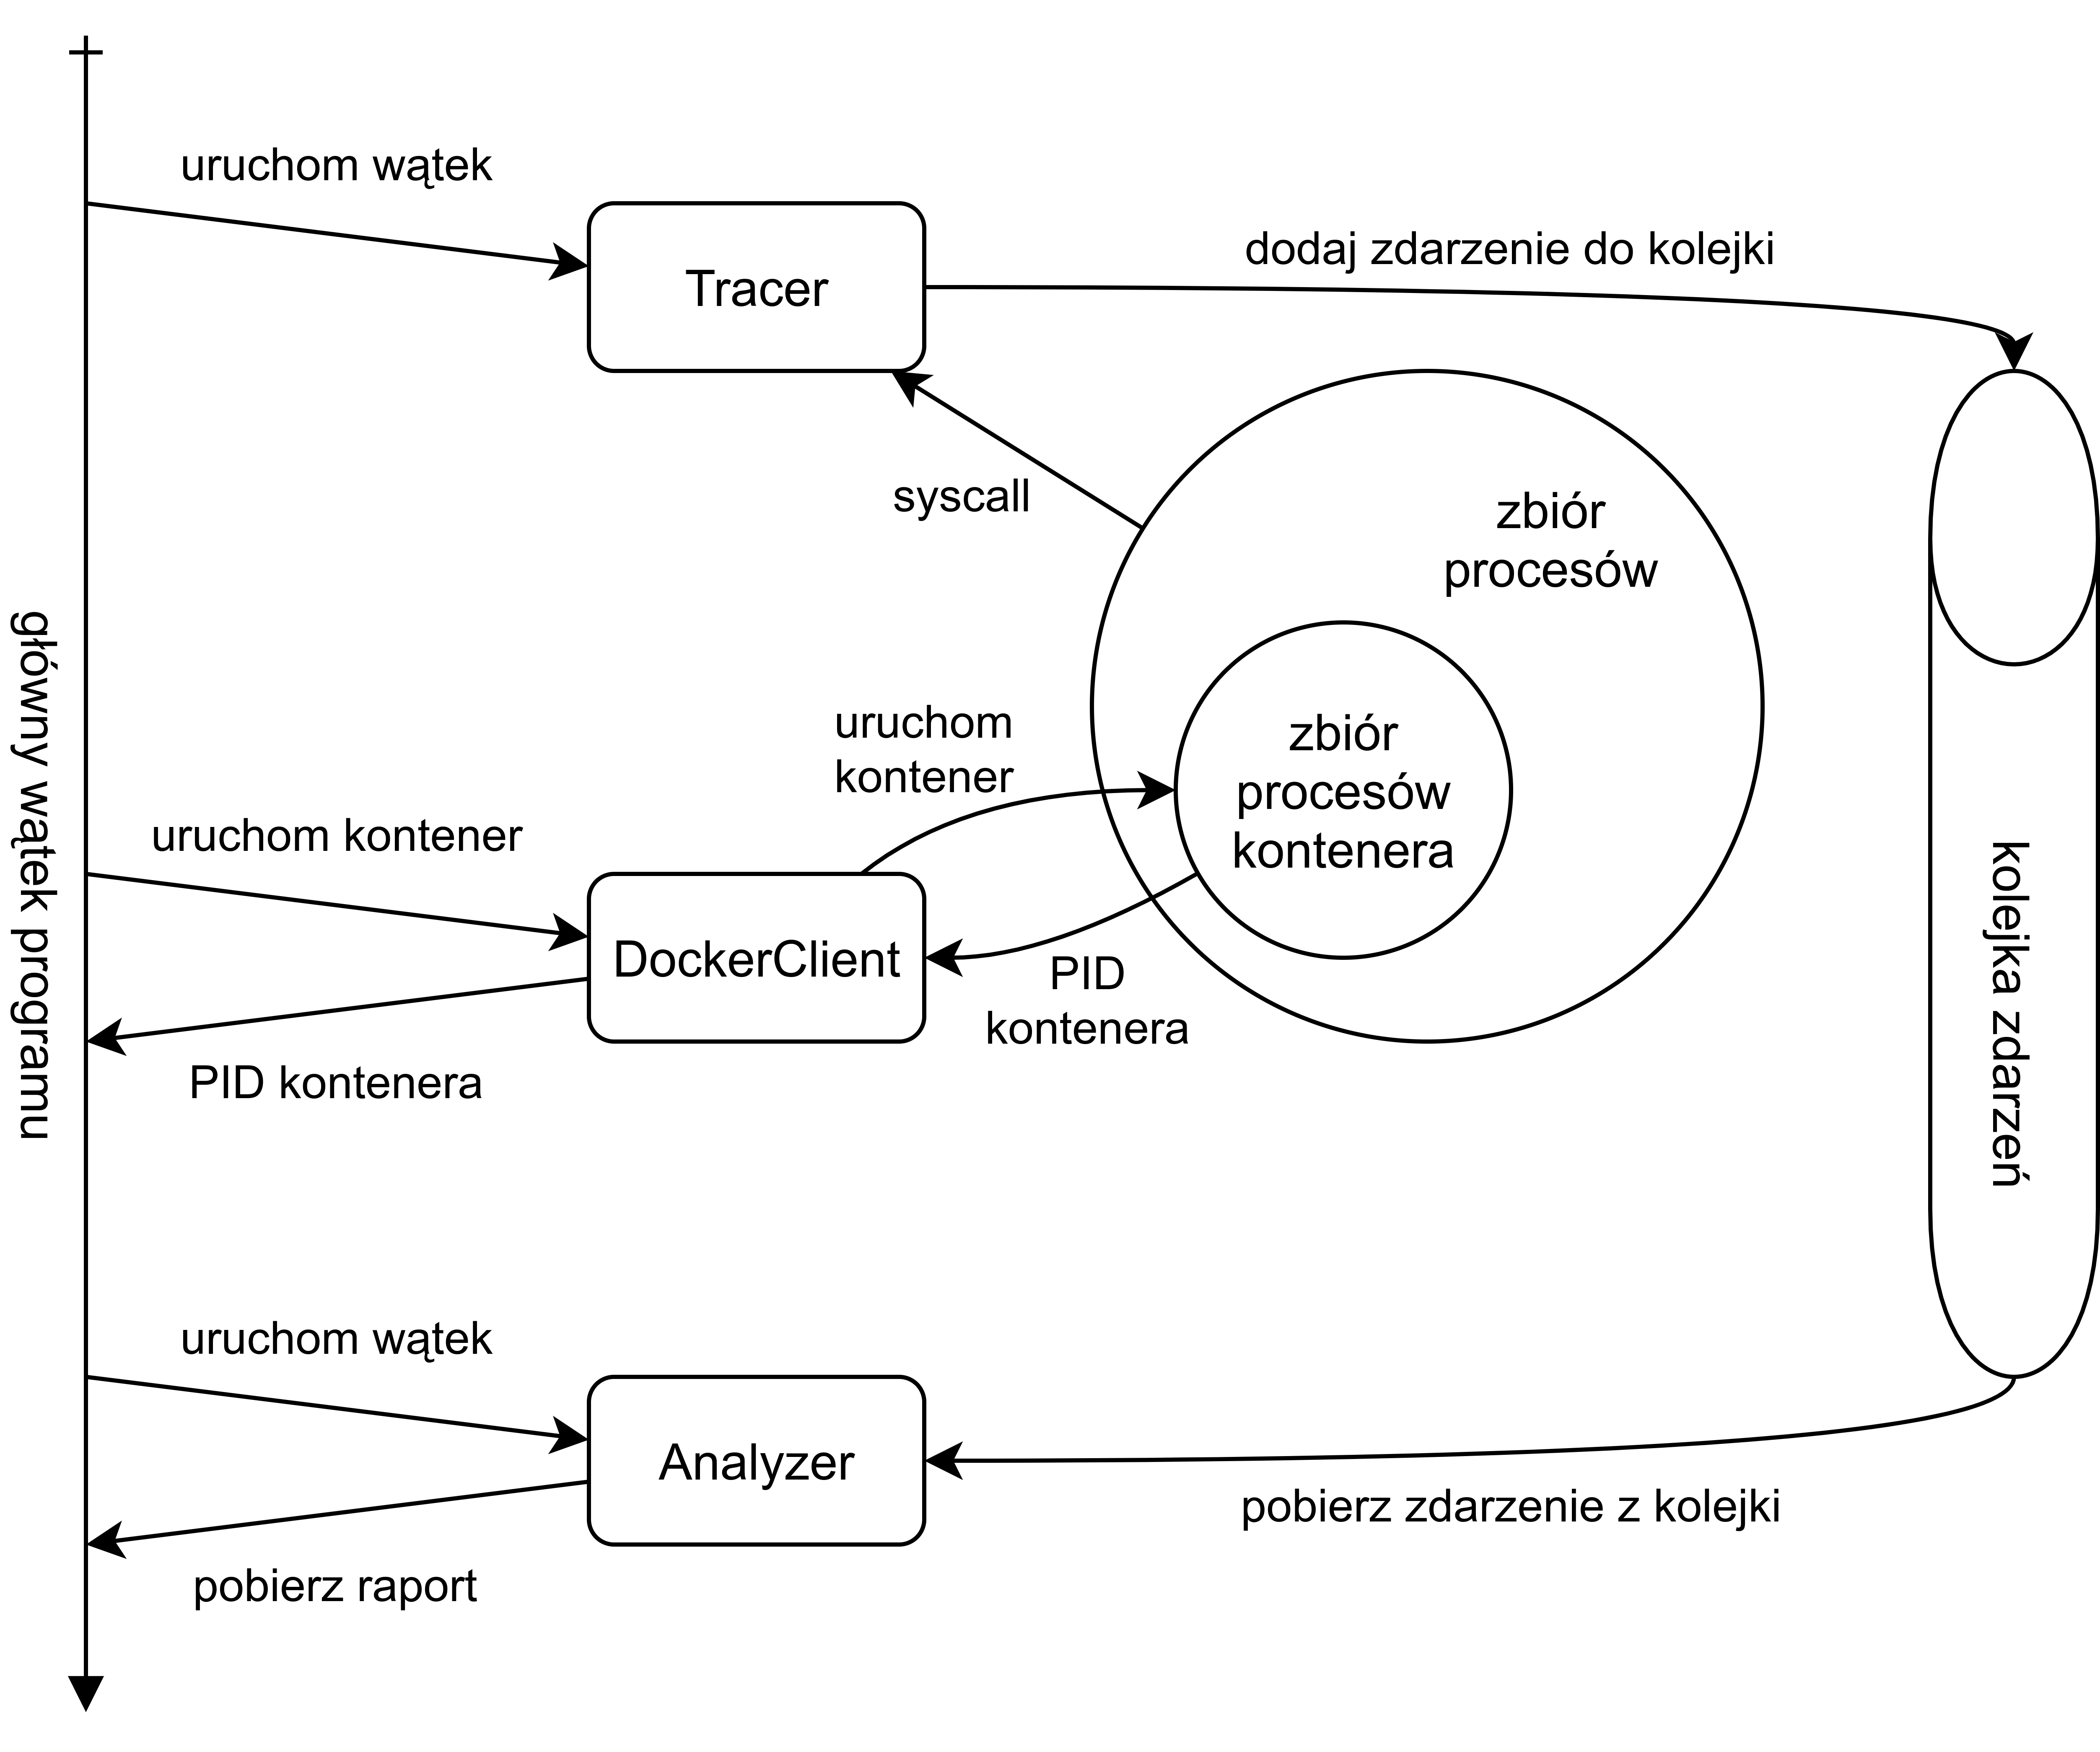
\includegraphics[width=0.9\linewidth]{images/analyzerFlow.png}
    \caption{Schemat przepływu sterowania i~przepływu danych w analizatorze}
    \label{fig:analyzerFlow}
\end{figure}

\subsection{Parsowanie argumentów linii poleceń}

Analizator uruchamia się z~linii poleceń przy pomocy polecenia \textit{python3.7 main.py $<$image$>$}. Program akceptuje również te same opcje, które można przekazać do polecenia \textit{docker run} w~trakcie uruchamiania kontenera. 

Klasa \textit{Parser} implementuje obsługę opcji narzędzia Docker przy pomocy klasy \textit{ArgumentParser} z~modułu \textit{argparse}. Niemożliwe było wykorzystanie oryginalnego kodu źródłowego interfejsu linii poleceń Dockera, gdyż tak samo jak silnik i~demon Dockera, jest on napisany w~języku Go. Wzięty pod uwagę był również parser narzędzia Docker Compose napisanego w~Pythonie, który pozwala na definicję wielokontenerowych aplikacji Dockera w~formacie pliku YAML. Niestety, Docker Compose pozwala na zadeklarowanie dodatkowej konfiguracji, która jest niedostępna w~ramach polecenia uruchomienia kontenera. Co więcej, format zakłada inną składnię opcji, więc wymagane byłoby mapowanie pomiędzy standardami Docker SDK for Python, a~Docker Compose. Tym samym, najprostszym rozwiązaniem było stworzenie parsera od zera.

\subsection{Uruchomienie kontenera}

Kontener zostaje uruchomiony w~głównym wątku programu poprzez obiekt klasy \textit{ContainerManager}, która opakowuje obiekt klasy \textit{DockerClient} z~modułu \textit{docker}. Opcje uzyskane z~parsera zostają przekazane do wywołania metody \textit{run}, która zwraca obiekt klasy \textit{Container}. Obiekty tej klasy reprezentują stan kontenera w~danym momencie czasu. Wywołanie metody \textit{reload} powoduje wczytanie obecnego stanu kontenera. Początkowo, zwrócony obiekt nie posiada globalnego identyfikatora procesu punktu wejściowego kontenera (zwanego dalej, dla uproszczenia \textbf{identyfikatorem procesu kontenera}). Dlatego też, metoda \textit{start} obiektu klasy \textit{ContainerManager} odświeża obiekt kontenera do momentu uzyskania identyfikatora procesu kontenera, a~następnie zwraca tę wartość.

\subsection{Śledzenie wywołań systemowych}

Śledzenie wywołań systemowych odbywa się w~osobnym wątku, który jest uruchamiany poprzez obiekt klasy \textit{CapabilitiesTracer}. Metoda \textit{start} wykorzystuje klasę \textit{BPF} z~modułu \textit{bcc} narzędzia BCC w~celu skompilowania programu eBPF napisanego w~języku C++. Program eBPF zawiera w~sobie funkcję \textit{kretprobe__cap_capable}, która poprzez BCC zostaje załadowana do modułu BPF w~jądrze. Dzięki temu, zostanie ona wywołana po każdym wywołaniu funkcji systemowej \textit{cap_capable}, która służy do sprawdzenia czy dany proces posiada określone uprawnienie. Funkcja \textit{kretprobe__cap_capable} poprzez argumenty posiada dostęp do kontekstu wywołania systemowego \textit{cap_capable}: uprawnienia i~stanu procesu, którego zapytanie dotyczy oraz wartości zwróconej z~funkcji.

BCC udostępnia funkcję \textit{bpf_get_current_task}, która zwraca strukturę zawierającą informacje dotyczące procesu, w~którym doszło do wywołania systemowego. W~strukturze tej znajduje się identyfikator procesu (\textit{.pid}) oraz wskaźnik na strukturę tego samego typu dotyczącą rodzica (\textit{.parent}). Iterując po wskaźnikach w~górę drzewa procesów można sprawdzić czy wywołanie dotyczyło jednego z~procesów kontenera. Jednakże, ograniczenia programów eBPF zabraniają wykorzystania pętli w~kodzie bajtowym. Dlatego też skorzystano z~metody odwijania pętli (ang.~loop unrolling, loop unwinding), która zamienia pętlę na określoną liczbę następujących po sobie bloków wewnętrznych pętli. Oznacza to również, że liczba "iteracji" musi być z~góry określona i~ograniczona. Tym samym, istnieje możliwość wywołania systemowego \textit{cap_capable} wewnątrz kontenera, które nie zostanie wykryte przez program eBPF.

Komunikacja programu eBPF z~analizatorem odbywa się poprzez obiekt tablicy stworzony przy pomocy funkcji \textit{BPF_PERF_OUTPUT} udostępnianej przez BCC. Obiekt korzysta z~bufora \textit{perf_output}, który pozwala na emitowanie zdarzeń z~przestrzeni jądra do przestrzeni użytkownika poprzez wywołanie na nim metody \textit{perf_submit}. Obiekt klasy \textit{CapabilitiesTracer} najpierw definiuje wywołanie zwrotne (ang.~callback) poprzez metodę \textit{open_perf_buffer} klasy \textit{BPF}, a~następnie oczekuje na zdarzenia przy pomocy metody \textit{perf_buffer_poll}. Załadowanie programu eBPF i~przepływ danych przedstawione są na rysunku \ref{fig:analyzerBPF}.

\begin{figure}[ht]
    \centering
    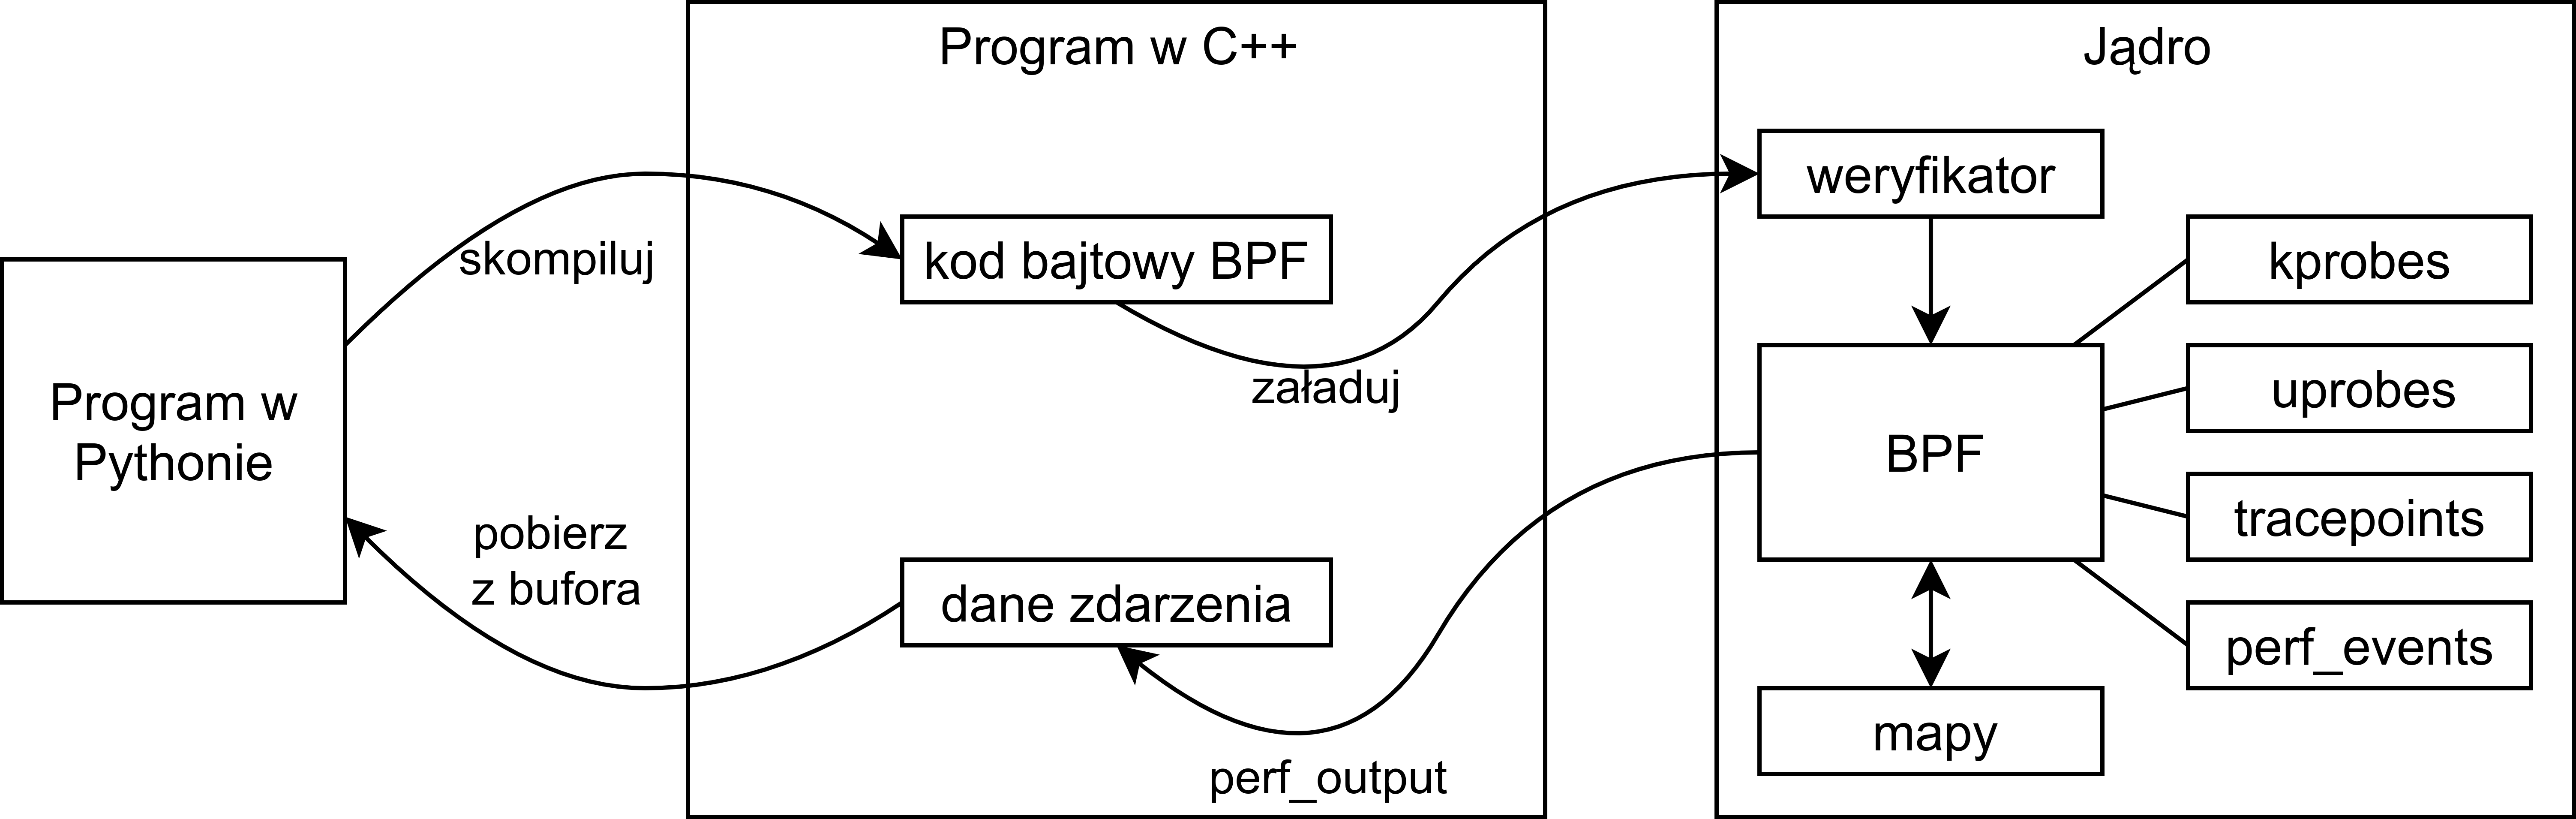
\includegraphics[width=0.9\linewidth]{images/analyzerBPF.png}
    \caption{Wykorzystanie narzędzia BCC w analizatorze}
    \label{fig:analyzerBPF}
\end{figure}

Jak już zostało wspomniane, program eBPF zostaje wykonany dla każdego wywołania systemowego \textit{cap_capable}. Należy określić sposób w~jaki odfiltrowane zostaną tylko te wywołania, które dotyczą procesów kontenera -- wyamaga to identyfikatora procesu kontenera. Zostały rozważone dwa poniższe warianty.

\subsubsection{Filtrowanie na poziomie programu eBPF}

Identyfikator procesu kontenera zostaje przekazany do programu eBPF przed kompilacją poprzez dyrektywę \textit{\#define}. Dzięki temu, program w~trakcie iteracji w~górę drzewa procesów może wykryć czy wywołanie dotyczyło kontenera i~tylko w~takim przypadku wyemitować zdarzenie. W~tym wariancie identyfikator procesu kontenera musi być znany jeszcze przed rozpoczęciem śledzenia. Oznacza to pewien okres czasu, w~którym kontener już działa, a~jego wykorzystanie uprawnień nie jest śledzone.

\subsubsection{Filtrowanie na poziomie analizy zdarzeń}

Każde wywołanie systemowe \textit{cap_capable} powoduje wyemitowanie zdarzenia. W~celu filtrowania na poziomie analizy zdarzeń, zdarzenie musi również zawierać cała gałąź drzewa procesów aż do procesu inicjującego (identyfikator procesu = 1). Gałąź drzewa procesów zapisywana jest w~postaci tablicy identyfikatorów procesów, gdzie każdy element oznacza identyfikator procesu, a~elementy ułożone są w~kolejności od dołu gałęzi drzewa. Należy przypomnieć, iż z~racji ograniczeń programów eBPF, cała gałąź drzewa procesów może nie zostać zapisana w~tablicy. Rysunek \ref{fig:analyzerPIDs} obrazuje metodę powstawania tablicy.

\begin{figure}[ht]
    \centering
    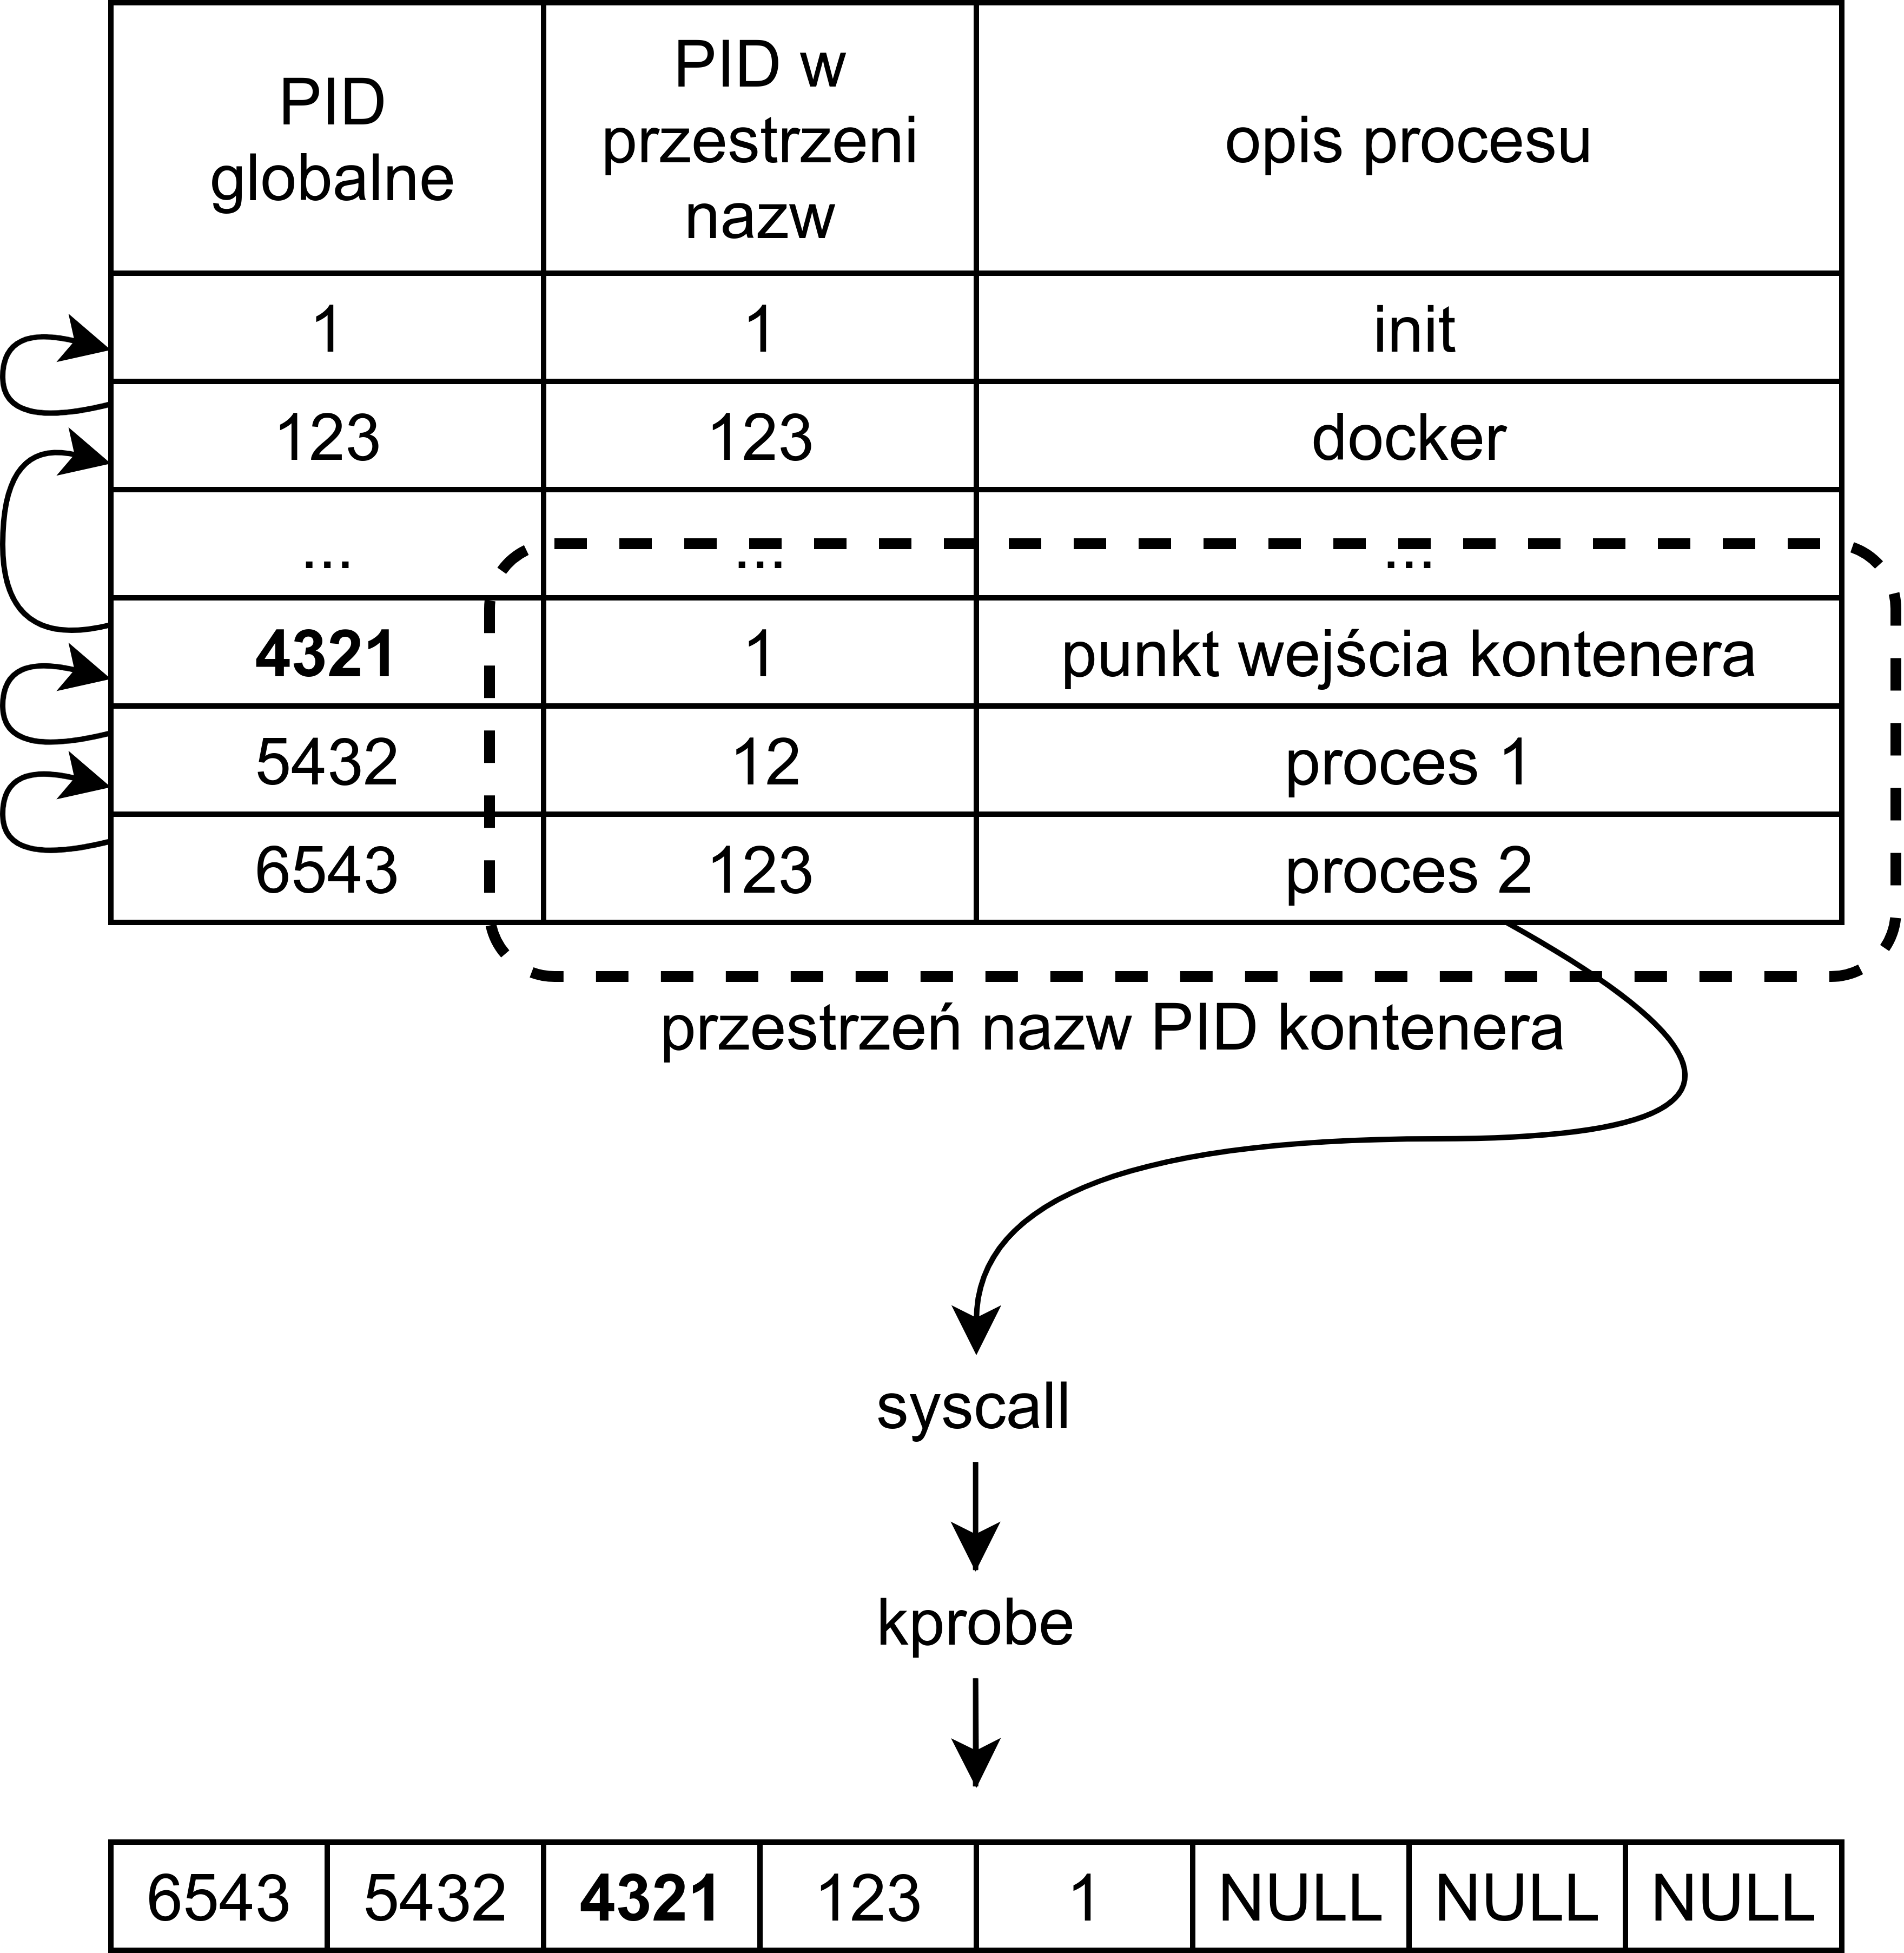
\includegraphics[width=0.9\linewidth]{images/analyzerPIDs.png}
    \caption{Schemat powstawania tablicy gałęzi drzewa procesów}
    \label{fig:analyzerPIDs}
\end{figure}

\subsubsection{Wybór wariantu}

Wybór pomiędzy dwoma wariantami opierał się na kompromisie pomiędzy szybkością analizy, a~utratą początkowych wywołań systemowych kontenera. Warto zaznaczyć, że drugi wariant również może utracić część wywołań z~powodu zbyt dużej ich ilości. Jądro może nie uruchomić programu eBPF dla zbyt szybko pojawiających się wywołań systemowych lub bufor \textit{perf_output} może się zapełnić prowadząc do utraty zdarzeń. Dotyczy to również wariantu pierwszego, jednak w~mniejszym stopniu, gdyż ten wariant programu eBPF produkuje mniejszą ilość zdarzeń.

Ostateczna implementacja analizatora wykorzystuje filtrowanie na poziomie analizy zdarzeń. Pierwsze momenty od uruchomienia kontenera polegają najczęściej na inicjalizacji wewnętrznych usług, co w~dużej mierze prowadzi do wywołań systemowych. Informacja o~uprawnieniach wykorzystywanych w~trakcie inicjalizacji jest według autora relatywnie ważniejsza od możliwej utraty informacji z~późniejszych wywołań systemowych.

Wywołanie zwrotne odczytujące zdarzenia z~bufora przekształca je w~obiekt klasy \textit{CapabilityEvent}, a~następnie dodaje do kolejki zdarzeń typu \textit{Queue} z~modułu \textit{queue}. Klasa \textit{Queue} implementuje wymagane zabezpieczenia synchronizacyjne dzięki czemu może być użyta w~aplikacjach wielowątkowych. Ponadto, przepływ elementów odbywa się w~porządku FIFO (ang.~first-in, first-out).

\subsection{Analiza wywołań systemowych}

Analiza wywołań systemowych również odbywa się w~osobnym wątku, który jest uruchamiany poprzez obiekt klasy \textit{CapabilitiesAnalyzer}. Obiekt tej klasy wykorzystuje konfigurację odczytaną z~obiektu klasy \textit{Container} w~celu zdefiniowania zbioru uprawnień udzielonych kontenerowi. Obiekt pasywnie czeka na zdarzenia pojawiające się w~kolejce. Dla każdego ze zdarzeń sprawdza jego gałąź identyfikatorów procesów. Jeśli zdarzenie dotyczy procesu wewnątrz kontenera to w~zależności od tego, czy uprawnienie zostało udzielone przez jądro czy nie, dodaje je do odpowiedniego zbioru, 

\subsection{Zwolnienie zasobów i~zakończenie programu}

Program analizatora kończy się w~momencie zakończenia pracy kontenera bądź wymuszenia zakończenia przez użytkownika. Jeśli to użytkownik wymusił zakończenie programu kontener zostaje zastopowany. Główny wątek analizatora nastepnie wysyła sygnał do wątków wewnątrz obiektów klas \textit{CapabilitiesTracer} i~\textit{CapabilitiesAnalyzer} aby zakończyły działanie. Obiekt klasy \textit{CapabilitiesTracer} kończy śledzenie wywołań systemowych natychmiastowo, zaś obiekt klasy \textit{CapabilitiesAnalyzer} najpierw odczytuje i~analizuje wszystkie zdarzenia pozostałe w~kolejce, a~następnie wyświetla raport dotyczący uprawnień.

Raport bazuje na opcjach zmieniających uprawnienia, przekazanych do kontenera w~trakcie uruchomienia analizatora:
\begin{itemize}
    \item \textit{-{}-cap-add}
    \item \textit{-{}-cap-drop}
    \item \textit{-{}-privileged}
\end{itemize}
oraz na uprawnieniach, które procesy kontenera próbowały użyć w~trakcie działania -- wywołania systemowe \textit{cap_capable}. Raport składa się z~4 sekcji, przedstawiających zbiory uprawnień:
\begin{itemize}
    \item "declared" -- przypisane do kontenera uprawnienia
    \item "granted" -- przypisane do kontenera uprawnienia, z~których skorzystał w~trakcie analizy
    \item "declared but not granted" -- przypisane do kontenera uprawnienia, z~których nie skorzystał w~trakcie analizy
    \item "not granted" -- uprawnienia, z~których kontener chciał skorzystać w~trakcie analizy, ale nie miał ich przypisanych
\end{itemize}

Głównym celem analizy jest zbiór uprawnień "declared but not granted", który obrazuje zjawisko udzielenia nadmiarowych uprawnień kontenerowi (ang.~over permissioning). Oczywiście, analiza była dokonywana w~trakcie działania kontenera, co oznacza, że najprawdopodobniej nie wszystkie ścieżki wykonania kodu zostały wykorzystane. Jednakże, ten zbiór uprawnień zawiera potencjalnych kandydatów do użycia z~opcją \textit{-{}-cap-drop}. Ciekawy również jest ostatni zbiór uprawnień -- "not granted" -- zawarte w~nim uprawnienia próbowały zostać wykorzystane przez kontener jednak nie posiadał on do tego zgody.

\section{Wyniki przykładowej analizy}

Analizator został uruchomiony dla obrazu \textit{postgres:latest}, a~kontener poza domyślnymi uprawnieniami otrzymał dodatkowe uprawnienie \textit{SYS\_TIME} oraz zostało mu odebrane uprawnienie \textit{KILL}:
\begin{verbatim}
python3.7 main.py --cap-add SYS_TIME --cap-drop KILL postgres:latest
\end{verbatim}
Zwrócony został poniższy raport:
\begin{verbatim}
Container declared capabilities:
         AUDIT_WRITE
         CHOWN
         DAC_OVERRIDE
         FOWNER
         FSETID
         MKNOD
         NET_BIND_SERVICE
         NET_RAW
         SETFCAP
         SETGID
         SETPCAP
         SETUID
         SYS_CHROOT
         SYS_TIME
Container granted capabilities:
         CHOWN
         DAC_OVERRIDE
         FOWNER
         FSETID
         MKNOD
         SETGID
         SETPCAP
         SETUID

Container declared but not granted capabilities (over permissioning):
         AUDIT_WRITE
         NET_BIND_SERVICE
         NET_RAW
         SETFCAP
         SYS_CHROOT
         SYS_TIME

Container not granted capabilities (under permissioning):
         SYS_ADMIN
\end{verbatim}

W celu poprawy bezpieczeństwa warto byłoby przeanalizować użycie przez kontener następujących uprawnień: \textit{AUDIT\_WRITE}, \textit{NET\_BIND\_SERVICE}, \textit{NET\_RAW}, \textit{SETFCAP}, \textit{SYS\_CHROOT}, \textit{SYS\_TIME} i~w miarę możliwości odebrać mu te, które są przez niego niewykorzystywane.